\documentclass{article}

\usepackage[utf8]{inputenc}
\usepackage{scrextend}
\usepackage{graphicx}
% Margins
\topmargin=-0.45in
\evensidemargin=0in
\oddsidemargin=0in
\textwidth=6.5in
\textheight=9.0in
\headsep=0.25in
\graphicspath{ {./} }

\title{Progetto di Automated Reasoning\\2021-2022}

\author{ Christian Londero }
\date{15 Febbraio 2022}

\begin{document}
\maketitle

\section{Definizione del problema}
Si consideri una scacchiera $n$ x $n$ ($n$ è dato in input). Si hanno a disposizione $l$ pezzi a forma di L, $s$ pezzi a forma di quadrato e $r$ pezzi a forma di rettangolo (si veda la figura, la dimensione del rettangolo è 3 x 1, il quadrato è 2 x 2 e il lato lungo della L è 2). $l$, $s$, $r$ sono dati in input. L'obbiettivo è di riempire la scacchiera con i pezzi a disposizione in maniera tale da minimizzare le celle vuote/free. Il requisito aggiuntivo è che $f$ celle (date in input) siano già occupate (quindi vietate).\\
Si veda l'esempio (le celle grigie sono già occupate/vietate).

\subsection{Considerazioni}
Si presenterà un algoritmo che tenta di minimizzare le celle empty scegliendo da un sottoinsieme dei pezzi. \\
Quindi si può dare in input un numero molto alto di pezzi al fine di "semplificare" la minimizzazione, sebbene si rischia in questo caso di fare utilizzare gli stessi tipi di pezzi quasi ovunque.\\
Nella sezione dei risultati vedremo infatti che se abbiamo a disposizione un elevato numero di pezzi ($3*l + 4*s + 3*r \gg n*n$) allora il solving è "facile", rispetto a un numero quasi giusto di pezzi ($3*l + 4*s + 3*r \simeq n*n$).

\section{Soluzione in minizinc}
Il programma che risolve il problema è \textit{main.mzn}.\\
Prende in input i seguenti parametri:
\begin{itemize}
    \item \textit{n} (intero): dimensione della board;
    \item \textit{l} (intero): numero di L (2x2) disponibili;
    \item \textit{s} (intero): numero di quadrati (2x2) disponibili;
    \item \textit{r} (intero): numero di rettangoli (1x3) disponibili;
    \item \textit{f} (intero): numero di celle vietate/forbidden/già occupate;
    \item \textit{forbidden} (array): array lungo $f$ di coordinate $X,Y$.
\end{itemize}
La board è una matrice (array bi-dimensionale) $n$ x $n$ il cui dominio è definito dalla seguente enumerazione: XXX, EEE, S11, S12, S13, S14, R11, R12, R13, R21, R22, R23, L11, L12, L13, L21, L22, L23, L31, L32, L33, L41, L42, L43.\\
Al fine di rendere comprensibile l'enumerazione si osservi la figura qui di seguito.\\
\begin{figure}[h!]
    \centering
    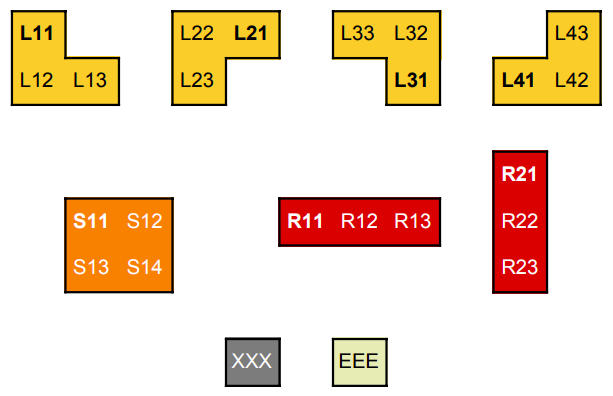
\includegraphics[width=0.7\textwidth]{shapes}
    \caption{Tutte le possibili shapes con rotazioni}
\end{figure}
Quindi ogni cella può assumere uno di quei valori dell'enumerazione, si è quindi proceduto a definire dei vincoli che mantengano le forme corrette.
\end{document}